\documentclass[12pt]{report}
\usepackage[a4paper]{geometry}
\usepackage{fancyhdr}
\usepackage{lastpage}
\usepackage{graphicx, wrapfig, subcaption, setspace, booktabs}
\usepackage[T1]{fontenc}
\usepackage[font=small, labelfont=bf]{caption}
\usepackage{fourier}
\usepackage[protrusion=true, expansion=true]{microtype}
\usepackage[english]{babel}
\usepackage{sectsty}
\usepackage{url, lipsum}
\usepackage{enumitem}
\usepackage{float}

\restylefloat{table}
\graphicspath{ {img/} }
\newcommand{\HRule}[1]{\rule{\linewidth}{#1}}
\renewcommand{\headrulewidth}{0pt}
\linespread{2}

%-------------------------------------------------------------------------------
% HEADER & FOOTER
%-------------------------------------------------------------------------------
% \pagestyle{fancy}
% \fancyhf{}
% \fancyhead[L]{Student ID: 20550430}
% \fancyhead[R]{University of Waterloo}
% \fancyfoot[C]{\thepage} % / \pageref{LastPage}

%-------------------------------------------------------------------------------
% TITLE PAGE
%-------------------------------------------------------------------------------

\begin{document}
\begin{titlepage}
   \begin{center}
    	\normalsize \textbf{\uppercase{University of Waterloo}} \\
		Faculty of Mathematics \\
	\end{center}	
		\vspace*{\stretch{0.1}}
	\begin{center}
		\HRule{0.5pt}
   		\LARGE \textbf{\uppercase{Introduction to Machine Learning in Finance: Applications \& Implications}}
   		\HRule{0.5pt}
	\end{center}
	\vspace*{\stretch{0.1}}
	\begin{center}
	   		\normalsize {TD Asset Management\\ Toronto, Ontario}	
	 
	\end{center}
	\vspace*{\stretch{0.1}}
	\begin{center}
	   		\normalsize {Prepared by\\
				Nicholas Westbury\\
				3B Computer Science\\
				ID 20550430\\
	   		 	\today
	   		 }
	\end{center}
\end{titlepage}

\newpage\noindent\thispagestyle{empty}
\LARGE\textbf{\uppercase{MEMORANDUM}} \normalsize
\vspace*{-10px}
\begin{singlespacing}\noindent
\vspace*{-10px}
To: TDAM Manager\\
\vspace*{-10px}
From: Nicholas Westbury\\
\vspace*{-10px}
Date: \today\\
\vspace*{-10px}
Re: Work Report: Introduction to Machine Learning in Finance \\
\end{singlespacing}
\HRule{1.5pt}\\
I have prepared the enclosed report, "Introduction to Machine Learning in Finance: Application \& Implications" for my 3B work report. This is the third of four work reports that the Co-operative Education Program required as part of Co-op degree requirements. As you are aware, my primary duty this work term was to support the portfolio analytics web tool. This report is an exploration of a potentially disruptive technology to this industry.\\ \\ \noindent
As part of this process, the Faculty of Mathematics requests that you evaluate this report for command of topic and technical content/analysis. Your evaluation will be submitted to the Math Undergrad Office for evaluation. The combined marks determine whether the report will receive credit. \\ \\
Thank you for your help in preparing this report,\\ \\ \noindent

\includegraphics[scale=0.55]{signature}

\newpage\thispagestyle{fancy}\sectionfont{\scshape}
\section*{\centering Table of Contents}
\normalsize
\begin{enumerate}[label={},leftmargin=*,labelsep=2ex]
    \item 1.0 Introduction \dotfill 1
    \item 2.0 Analysis \dotfill 2
    \item 2.1 Applications \dotfill 2
      \begin{enumerate}[label*={},leftmargin=*,labelsep=2ex]
        \item 2.1.1 Customer Service \dotfill 2
        \item 2.1.2 Fraud Detection \dotfill 3
        \item 2.1.3 Portfolio Analysis \dotfill 3
      \end{enumerate}
    \item 2.2 Active Portfolio Analysis \dotfill 5
    \begin{enumerate}[label*={},leftmargin=*,labelsep=2ex]
    	\item 2.2.1 Is portfolio optimization even possible? \dotfill 5
    \end{enumerate}
   	\item 2.3 Comparison of Algorithmic Methods \dotfill 6
    \begin{enumerate}[label*={},leftmargin=*,labelsep=2ex]
        \item 2.3.1 Linear Regression \dotfill 7
        \item 2.3.2 Support-Vector Machine \dotfill 8
        \item 2.3.3 Neural Network \dotfill 9
        \item 2.3.4 Evolution Algorithms \dotfill 10
      	\item 2.3.5 Summary of comparisons \dotfill 11
    \end{enumerate}
    \item 3.0 Conclusion \dotfill 12
    \item 4.0 References \dotfill 13
\end{enumerate}
\fancyfoot[C]{ii}

\newpage\thispagestyle{fancy}\sectionfont{\scshape}
\section*{\centering List of Figures}
\normalsize\cfoot{3aa}
\begin{enumerate}[label=\arabic*,leftmargin=*,labelsep=2ex,ref=\arabic*]
    \item Linear Regression Graph \dotfill 8
    \item Neural Network Nodes \dotfill 9
    \item Comparison Table \dotfill 11
    \item Algorithm Adoption Graph \dotfill 12
\end{enumerate}

\fancyfoot[C]{iii}

\newpage\thispagestyle{fancy}\sectionfont{\scshape}
\section*{\centering Executive Summary}

This report looks at the potential applications, both present and future, of machine learning in finance. It explores deeper the particular task of portfolio optimization. It considers four algorithms: linear regression, evolution, support-vector machine, and neural networks for the portfolio optimization task and gives a high-level overview of their functionality, comparing some of their advantages and disadvantages.

After reading this report, the reader should have a basic understanding of what machine learning is, how some particular algorithms work, and some of the considerations that goes into developing tools to solve this particular task such as the type of data used and how data is classified from the raw input data. In conclusion, you'll understand the importance of machine learning and why their adoption has been trending upwards.

\fancyfoot[C]{iv}

%-------------------------------------------------------------------------------
% BODY
%-------------------------------------------------------------------------------

\newpage\thispagestyle{fancy}\sectionfont{\scshape}

% Reset the page counter
\setcounter{page}{1}
\fancyfoot[C]{\thepage}

\section*{\centering 1.0 Introduction: What is Machine Learning?}
\addcontentsline{toc}{section}{Introduction}
\par\indent
Quantitative data has always been a core pillar of the finance industry. From hedge funds using a variety of numeric indicators to predict an economy's health to accountants calculating companies' output, the finance industry has been intrinsically linked with numbers. Traditionally, human workers have manually used these numbers to inform their decisions, such as whether to buy or sell an asset or the amount of risk to take. Given the ever-increasing quantity of data, making good decisions is a difficult task. The sector is therefore a natural target for applying algorithms to systemically organize and analyze information.
\\ \par\noindent
One relatively recent advancement in algorithmic analysis has been labeled "Machine Learning". In short, machine learning the application of statistical and optimization methods to recognize and learn from patterns in data. Algorithms can range dramatically in sophistication from linear regression, classifying data based on if it falls above or below a threshold, to neural networks, layers of nodes that each learn about increasingly abstract features of the data. This class of algorithms have a plethora of applications in all fields, but especially those dealing with quantification like finance. This report will explore some of the current applications, particularly stock analysis, and future implications of computational learning.

\newpage\thispagestyle{fancy}\sectionfont{\scshape}
\section*{\centering 2.0 Analysis}
\subsection*{\centering 2.1 Applications}
\noindent
There are variety of algorithm applications within the finance industry that offer considerable advantages over their human counterparts. Customer service, fraud detection, and portfolio-analysis are three of the primary which have been adopting machine learning techniques [1].

\subsection*{\centering 2.1.1 Customer Service}
\par\indent
One of the most promising applications of deep learning is in customer service. In particular, answering customers questions on a variety of topics can be highly automated. Chatbots, where customers ask questions that are processed in real-time and answered by an algorithm, are becoming increasingly accurate and popular. Questions like "what is my account balance" or "how to I open a TFSA" that would traditionally be answered by a bank teller can now be instead answered by a web service. The advantages are obvious; to the banks, they lower dependence on physical branches saving money on staff. To the customers, their questions are answered faster, more conveniently, and potentially more accurately. In the future, this will have an even greater presence. Gartner analytics predicts that 85\% of banking will happen through electronic means by 2020 [2].

\newpage\thispagestyle{fancy}\sectionfont{\scshape}
\subsection*{\centering 2.1.2 Fraud Detection}
\addcontentsline{toc}{section}{Introduction}
\par\indent
A second application where banks have already applied traditional algorithms for years is fraud detection. This is an important problem because despite only approximately 0.1\% of transactions being fraudulent, hundreds of millions of dollars are still lost to fraud every year [3].  In the recent past, credit card companies and other financial institutions set explicit flags to detect potentially suspicious activity, factors such as location and amount spend, which are often good potential indicators of fraud. Due to such low occurrences though, these methods are susceptible to false positives, when fraud is incorrect detected. Recently, more sophisticated machine learning algorithms can find correlations between transaction metrics that a hard-coded set of rules in flagging algorithms would miss and put less weight to less important factors. For example, a machine learning algorithm might find the frequency and location of transactions should be weighted as more important factors than amount and purchase type.


\subsection*{\centering 2.1.3 Portfolio Analysis}
\par\indent
A third popular application is to use machine learning algorithms to analyze portfolios. Different portfolios have different objectives from maximizing short-term returns to minimizing long-term risks. These types of optimization problems are well-suited for applying machine learning algorithms since the value function, return on investment, is clear. There is a considerable range of sophistication. The simplest form is closer to a passive investment strategy, where an algorithm allocates different a diversity of asset classes (e.g. stocks, bonds, currencies) based on risk tolerance. This is what popular robo-investing website like Wealthsimple, a Toronto start-up, offer because it minimizes risk.
\par\noindent \\
In addition to the passive investment strategy, algorithmic active asset selection is possible. These use financial metrics of an asset, such as earning per share, to evaluate whether an asset is under or overvalued and make trades based on these evaluations. Time-series analysis methods, where these metrics change over time is a common approach. Furthermore, algorithms can also be to take into account more abstract data such as sentiment analysis. Mentions of a particular the company in online articles or social media websites are analyzed to find the mood which people are talking about an asset or the overall economy. For example, if mentions generally use positive words when talking about an asset, it may be a good indicator that people are confident in the company. The remainder of this report will concentrate on explaining and comparing some of these algorithms.

\section*{\centering 2.2 Active Portfolio Analysis}
\subsection*{\centering 2.2.1 Is portfolio optimization even possible? }

Ever since financial markets where created, traders have been trying to find an edge to give them an advantage over others. Machine learning is just the latest iteration. There is a legitimate question of whether or not computational methods have good predictive power.
\par\noindent
One one hand, academia has consistently found that algorithms where generally on par with their benchmarks (generally a buy-and-hold strategy) [4][5]. This may suggest that either the data has weak predictive power or the market is "efficient", meaning it strongly reflects the data and therefore profit opportunities are marginal. Another reason the portfolio optimization problem is unsolved is that real-world data is imperfect, it can be expensive to access high-quality stock data for example, and even then accuracy will often be low.

On the other hand, as Clive Granger from the University of California points out there is a "possible reporting bias - if a method of forecasting found an academic might prefer to profit from it
rather than publish" [5]. To further support this point, Two Sigma and Renaissance, two of the world's largest hedge funds, actively employ data scientists. This type of hiring implies there is some value generation possible. Given the right tools, it is likely possible to take advantage of obscure patterns in data that the general investing public cannot.

\subsection*{\centering 2.2.2 Types of data}
For all machine learning methods, understanding the types of information available is particularly important. In finance, we have several types of data that is feed as input to the portfolio optimization algorithm: technical data, fundamental data, economic data, and sentimental data. Technical data refers to pricing data and related ratios like moving average price. Fundamental data refers to financial number generally released in quarterly reports such as earnings per share.  Economic data refers to economy-wide numbers like employment percentage which can reflect on individual companies. Finally there is sentimental data, this is generally collected from news articles or social media that relate a company to positive or negative emotions. Technical, fundamental, and economic data are the most commonly used due to its relatively-easy access. Pricing data is frequently updated making it a useful for machine learning application that require large amounts of data. Other types of data like fundamental data generally has more predictive power. The majority of portfolio analysis uses a time series analysis with technical data supplemented with other types of data.

\subsection*{\centering 2.3 Comparison of Algorithmic Methods}

We will consider a few different algorithmic approaches: regression, evolution, SVM, and ANN on the portfolio optimization problem. For each, a brief description of functionality will be given, some advantages and disadvantages will be discussed. Particular emphasis will be placed on evaluating their applications rather than their technical implementations.

\subsection*{\centering 2.3.1 Linear Regression}

Linear regression is one of the simplest forms of machine learning classifiers. Given an array of datapoints, linear regression tries to optimize an array of weights in order to minimize an error function between these labels. A frequently-used error function is simply the euclidean distance between points. Using this strategy, a hyperplane, simply a $n-1$ dimensional line in $n$-dimension space, is created.

This regression can then be used as a binary classifier where an asset datapoint is a undervalued if it falls below the regression or overvalued if above.  It can easily be extended to autoregression where time series data is used and we can predict future values. In practice, linear regression is used exclusively as a starting point for more complex price prediction strategies because the accuracy is generally lower. It does have the advantage of being simple and easy to interpret.

\begin{center}
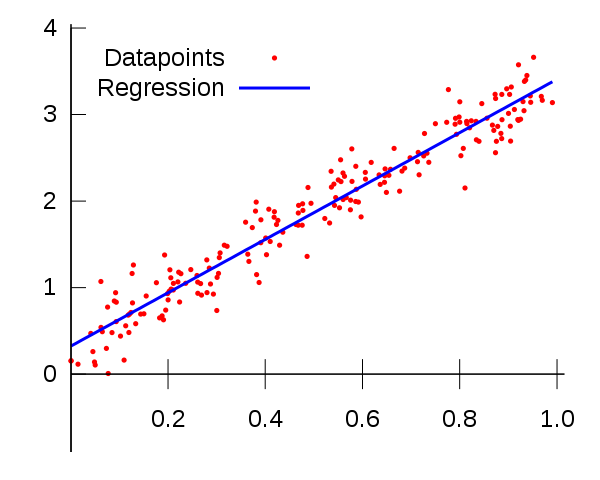
\includegraphics[scale=0.5]{linearregression}
\captionof{figure}{A 2-dimension linear regression [6]}
\end{center}

\subsection*{\centering 2.3.2 Support-Vector Machine}

Support-Vector Machines (SVM) are an extension of linear classifier. Like linear regression, they classify data into two classes. Without kernels, SVMs are identical to a linear classifiers. SVM differ from linear regression as they are more extensible. Kernels can added to allow differentiation of non-linear features. Adding these kernels can improve accuracy at the cost of potentially over-fitting the data by finding patterns in the data that don't generalize.

In terms of performance, SVMs are less computationally expensive to compute than neural networks and have been found to outperform in certain studies [5][7]. In addition, it generally takes less data to train. This makes SVMs strong candidates for situations with less data or computational resources are available.

\subsection*{\centering 2.3.3 Artificial Neural Networks}

Artificial Neural Networks (ANN) are the most complex classifier. They take inspiration from biological brains. On a high level, layers of nodes "neurons" are set up feeding into children nodes with different weights and activation levels. Generally the further the layer of node is from the original input data, the smaller the amount of nodes and the more abstract the features are. For example, an early layer node may activate on a high market capitalization and a later layer node may activate construct full portfolios. As with most of these algorithms, there are countless variations that can be tweaked, e.g. binary or continuous activation, connection limitations, feedforward-only etc. increasing performance somewhat. Some variations were found to outperform "buy \& hold" strategies by [5].

\begin{center}
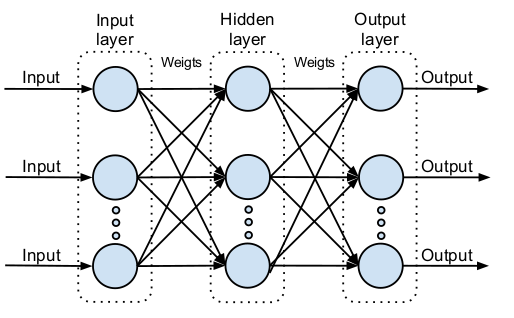
\includegraphics[scale=0.5]{ANN}
\captionof{figure}{A sample of three neuron layers, the input layer is the raw data and the output layer is the final result with hidden layers increasing data abstraction. [5]}
\end{center}

\newpage
\subsection*{\centering 2.3.4 Evolution Algorithms}

A class of algorithms that is also inspired from nature, this time from biological evolution are evolution algorithms. They can be useful for search problems where a large search space needs to be efficiently explored. Often they are used not as a portfolio-optimizer but as a parameter optimizer for other algorithms like ANNs. They work by starting with an initial generation of parameters and randomly mutate these parameters at each generation with a value function to eliminate generations with lower values, similar to natural selection. In some variations, there is an additional "cooling factor" where later generations vary less than earlier generations as optimality is approached. 

\newpage
\subsection*{\centering 2.3.5 Comparison of algorithms}

These four algorithm classes are appropriate for certain aspects of the portfolio optimization task. The evolution algorithm is generally used for parameter optimization wheres the other algorithms linear regression, SVM, and ANN are used to optimize portfolio holdings. Given certain constraints of a task, certain tools may be more useful. For example, high-frequency traders might favor SVM given the time-constraints whereas long-term traders may favor ANN for its often higher accuracy.\\

\begin{figure}[H]
   \centering % center the table
   \begin{tabular}{ |c|c|c|c| }
 	\hline
 	\textbf{Model} & \textbf{Implementation Ease} & \textbf{Uses} & \textbf{Performance} \\ \hline
 	Linear Regression & Easy & Optimization, Benchmark & Low \\ 	\hline
 	Evolution & Easy & Parameter Optimization & Fair \\ \hline
 	SVM & Medium & Optimization & High \\ \hline
 	ANN & Complex & Optimization & High \\ \hline
	\end{tabular}
	\caption{Comparison of popular optimization algorithms for the portfolio optimization task}
\end{figure}

\newpage\thispagestyle{fancy}\sectionfont{\scshape}
\section*{\centering 3.0 Conclusion}
\addcontentsline{toc}{section}{Conclusion}
\par\noindent
As all domains increase their dependence on cutting-edge technologies, it's inevitable that the finance domain continues a transition from human to computer decision making. Machine learning has already been applied to customer service and fraud detection, and their scope will inevitable be expanded in the near future. Portfolio optimization is a difficult problem and academia has a mixed-record on their algorithm performance. Still, some algorithms like SVM and ANN can perform better than benchmarks and it's probable that proprietary algorithms perform better still. Even today, traditional traders are slowly been replaced by trading algorithms. The advantages of using software include cutting costs, higher accuracy, and faster evaluation when compared to their human equivalents. \\

\begin{center}
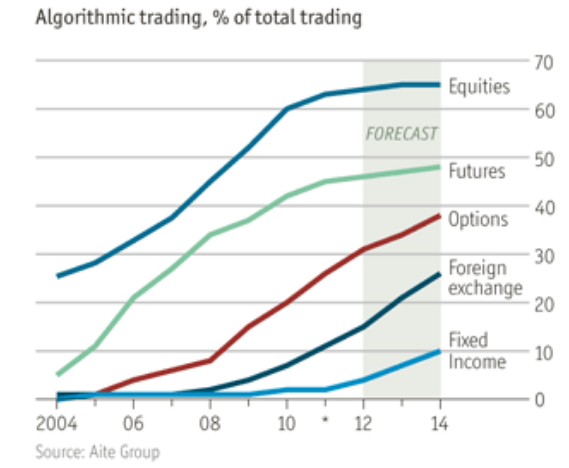
\includegraphics[scale=0.4]{autotrade}
\captionof{figure}{All types of trading are increasingly been done by algorithms. [8]}
\end{center} 

 \noindent

%-------------------------------------------------------------------------------
% REFERENCES
%-------------------------------------------------------------------------------
\newpage
\section*{\centering 4.0 References}
\addcontentsline{toc}{section}{References}

\begin{enumerate}
\item Faggella, Daniel. "Machine Learning in Finance - Present and Future Applications." TechEmergence, 25 Aug. 2017.
\item Gartner Analytics. "CRM Strategies and Technologies to Understand, Grow and Manage Customer Experiences", 2 Feb. 2011
\item Lisboa, P. J. G., et al. Business applications of neural networks: the state-of-the-Art of real-World applications. World Scientific, 2000.
\item Andersen, Andre et Mikelsen, Stian. "A Novel Algorithmic Trading Framework Applying Evolution and Machine Learning for Portfolio Optimization". Norwegian University of Science and Technology, 2012.
\item Granger, Clive W.J. Forecasting stock market prices: Lessons
for forecasters. International Journal of Forecasting, 1992.
\item Fumo, David. "Linear Regression - Intro To Machine Learning." Medium. Simple AI, 05 Mar. 2017. Web. 16 Dec. 2017.
\item P Pai, W Hong. Forecasting regional electricity load based on recurrent support vector machines. Electric Power Systems
Research, June 2005.
\item "The fast and the furious." The Economist, The Economist Newspaper, 25 Feb. 2012, www.economist.com/node/21547988.
\end{enumerate}

\end{document}